\documentclass{beamer}
\usepackage[utf8]{inputenc}
\usetheme{Warsaw}

\usepackage{tikz,tkz-tab}

\newtheorem{proposition}{Proposition}
\newtheorem{exemple}{Exemple}

\title{Second degré.}
%\author{B. Meuhr}\institute{École Normale Supérieure, département de pipologie}

\begin{document}
  
  \begin{frame}
    
    \titlepage
    
  \end{frame}
  
  
    
  \section{Fonctions polynômes de degré 2.}
  \begin{frame} 
    
  \begin{definition}
    \begin{itemize}
     \item Une \textbf{fonction polynôme de degré 2} est une fonction 
     $f$ définie sur $\mathbb{R}$ qui peut être mise sous la forme 
     \uncover<2,3,4,5,6>{$f(x)=ax^2+bx+c$ où $a,b,c$ sont trois nombres 
     rééls avec $a$} \uncover<3,4,5,6>{non nul.}
     
   \item L'expression $ax^2+bx+c$ est \uncover<4,5,6>{la \textbf{forme développée}} de $f(x)$.
     \item Une fonction polynôme de degré $2$ est aussi appelée 
     \uncover<5,6>{\textbf{trinôme} (du second degré).}
     \item On appelle \uncover<6>{\textbf{parabole}} la représentation graphique 
     d'un trinôme.
   \end{itemize}    
  \end{definition}
  
  \end{frame}
  
  \begin{frame}
    \begin{exemple}
    Les fonctions suivantes sont-elles des trinômes ?
    \begin{enumerate}
     \item $g(x)=2x^2+3x+1$. 
     \item $h(x)=3(x-1)^2+1$.
     \item $i(x)=4(x-1)(x+2)$.
     \item $i(x)=5x+3$.
     \item $j(x)=x^3+4x^2+1$.
     \end{enumerate}
  \end{exemple}
  \end{frame}
  
  \subsection{Trinôme du second degré.}
    
  \begin{frame}
    \begin{exemple}
      \begin{itemize}
      \item La fonction $g(x)=2x^2+3x+1$
      \uncover<2,3,4,5,6,7,8,9,10,11,12,13,14,15,16>{est un trinôme du second degré.}
      \item
      \uncover<3,4,5,6,7,8,9,10,11,12,13,14,15,16>{ La fonction $h(x)=3(x-1)^2+1$}
      \uncover<4,5,6,7,8,9,10,11,12,13,14,15,16>{est un trinôme du second degré.}
      \uncover<5,6,7,8,9,10,11,12,13,14,15,16>{En effet, $h(x)=$}
      \uncover<6,7,8,9,10,11,12,13,14,15,16>{$3(x^2-2x+1)+1=$}
      \uncover<7,8,9,10,11,12,13,14,15,16>{$3x^2-6x+4$.}
      \item 
      \uncover<8,9,10,11,12,13,14,15,16>{La fonction $i(x)=4(x-1)(x+2)$}
      \uncover<9,10,11,12,13,14,15,16>{est un trinôme du second degré.}
      \uncover<10,11,12,13,14,15,16>{En effet, $i(x)=$}
      \uncover<11,12,13,14,15,16>{$4(x^2-x+2x-1)=$}
      \uncover<12,13,14,15,16>{$4x^2+4x-4$.}
      \item 
      \uncover<13,14,15,16>{La fonction affine $i(x)=5x+3$}
      \uncover<14,15,16>{n'est pas un trinôme du second degré.}
      \item 
      \uncover<15,16>{Le polynôme $j(x)=x^3+4x^2+1$}
      \uncover<16>{n'est pas un trinôme du second degré.}
    
 \end{itemize}
     
 \end{exemple}
  \end{frame}  

  \subsection{Variations d'un trinôme du second degré}
  
  \begin{frame}
    \begin{theorem}
    Un trinôme, $f(x)=ax^2+bx+c$ admet pour variations:
    
    \begin{center}
     
    
    \resizebox{11cm}{!}
    {
      \begin{tabular}{c c}
      Si $a>0$	
       
      
      &
       Si $a<0$
      
      
      \\
      
      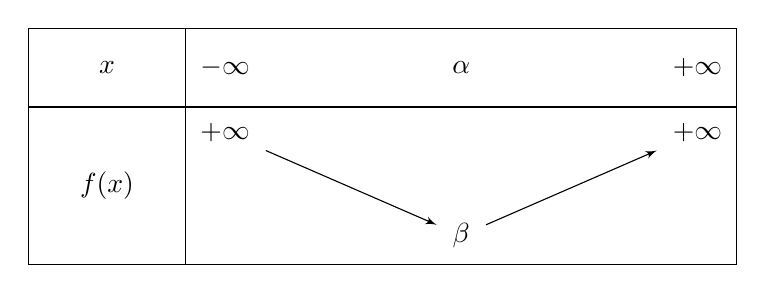
\begin{tikzpicture}
	\tkzTabInit{$x$ /1,$f(x)$/2}{$-\infty$, $\alpha$, $+\infty$}
	
	\tkzTabVar{+/$+\infty$,-/$\beta$,+/$+\infty$}
      \end{tikzpicture}
      &
      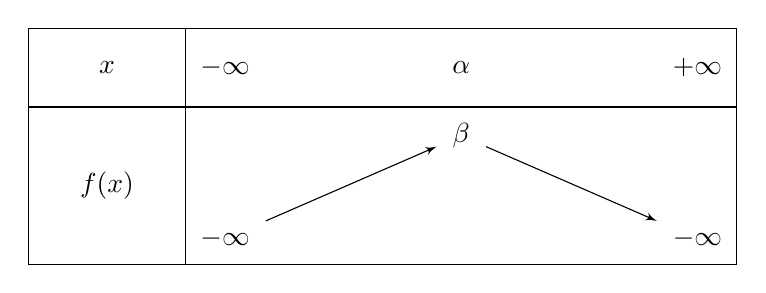
\begin{tikzpicture}
	\tkzTabInit{$x$/1,$f(x)$/2}{$-\infty$, $\alpha$, $+\infty$}
	
	\tkzTabVar{-/$-\infty$,+/$\beta$,-/$-\infty$}
      \end{tikzpicture}
      \end{tabular}
    }
    \end{center}
    
     On peut calculer les coordonnées $(\alpha,\beta)$ du sommet $S$ de la parabole grâce aux formules 
     $$\alpha=\uncover<2,3,4>{-\frac{b}{2a}} \hspace{1cm} \beta=\uncover<3,4>{f(\alpha)}$$
    
      De plus, $f$ s'écrit $f(x)=a(x-\alpha)^2+\beta$. Cette écriture est la
      \uncover<4>{\textbf{forme canonique}} du trinôme.
    \end{theorem}
  \end{frame}
  
    
  
  \begin{frame}
  \begin{exemple}
   Pour chacun des trinômes $P(x) = 2x^2+4x-3$ et $Q(x)=-(x-2)^2$ : 
   \begin{enumerate}
    \item Identifier les coefficients $a,b,c$.
    \item Dresser le tableau de variation.
  \end{enumerate}
 \end{exemple}
 \end{frame}
 
 \begin{frame}
   
   \begin{exemple}
   Pour chacun des trinômes $P(x) = 2x^2+4x-3$ et $Q(x)=-(x-2)^2$ : 
    \begin{enumerate}
    \item Identifier les coefficients $a,b,c$.
    \item Dresser le tableau de variation.
    \end{enumerate}
   \end{exemple}
 \end{frame}

 \begin{frame}
 Pour $P(x) = 2x^2+4x-3$, $a=2$, $b=4$, $c=-3$, comme $a$ est positif,
  $P$ est décroissant sur l'intervalle $]-\infty,\alpha]$ puis croissant
  sur l'intervalle $\alpha,\infty[$.
  
 \end{frame}

 
 
 \section{Racines et factorisation.}
 
 \begin{frame}
 \begin{definition}
    Soit $f(x)=ax^2+bx+c$ un trinôme du second degré et $\mathcal{P}$ sa représentation 
    graphique.
    
    On appelle \textbf{racines} de $f$ les solutions de l'équation \uncover<2,3>{$f(x)=0$}.
    Ce sont \uncover<3>{les abscisses} des points d'intersection entre $\mathcal{P}$ 
    et \uncover<3>{l'axe des abscisses}.
    
  \end{definition}
\end{frame}
  
  \begin{frame}
  \begin{exemple}
    Les fonctions suivantes admettent-elles des racines ? Si oui, combien ? 
    Et quelles sont-elles ?
    \begin{enumerate}
     \item $f(x)=3(x+1)(x-2)$. 
     \item $g(x)=2(x-3)^2$.
    \end{enumerate}
  \end{exemple}
\end{frame}
  
\begin{frame}
 
\end{frame}

\begin{frame}
  \begin{proposition}
   Soit $f(x)$ un trinôme du second degré et $\mathcal{P}$ sa représentation graphique.
    Trois cas peuvent se produire:
   
   \begin{itemize}
    \item $f$ admet $2$ racines, c'est-à-dire $\mathcal{P}$ 
    \uncover<2,3,4,5>{coupe l'axe des abscisses }en $2$ points.
    \item $f$ admet \uncover<3,4,5>{une racine}, c'est-à-dire $\mathcal{P}$
    est tangente à l'axe
    des abscisses ($1$ point d'intersection).
    
    Dans ce cas, on dit que la racine est une \uncover<4,5>{\textbf{racine double}}.
    
    \item $f$ n'admet pas de racine, c'est-à-dire $\mathcal{P}$ 
    \uncover<5>{ne coupe pas l'axe des abscisses}.
   \end{itemize}
   
  \end{proposition}
\end{frame}

\begin{frame}
 \begin{definition}[Discriminant]
    Soit $f(x)$ un trinôme du second degré dont la forme développée réduite
    est $f(x)=ax^2+bx+c$. On appelle \textbf{discriminant} de ce trinôme
    le nombre $\Delta=$\uncover<2>{$b^2-4ac$}.
    
  \end{definition}
  
  \begin{exemple}
    
    Calculer les discriminants des trinômes suivants:
    \begin{enumerate}
     \item Soit $h(x)=x^2-4x+3$.
     \item Soit $i(x)=2x^2-4x+2$.
     \item Soit $j(x)=-3x^2+12x-15$
    \end{enumerate}
   \end{exemple}
\end{frame}

\begin{frame}
 
\end{frame}


  \begin{frame}
    \begin{theorem}[Central]
    Soit $f(x)=ax^2+bx+c$ un trinôme.
    \begin{itemize}
      \item  si le discriminant $\Delta$ de $f(x)$ est 
      \uncover<2,3,4,5,6,7,8,9,10,11,12,13,14>{strictement positif} alors $f(x)$ admet deux racines :
      $$x_1=\uncover<3,4,5,6,7,8,9,10,11,12,13,14>{\frac{-b-\sqrt{\Delta}}{2a}} 
      \hspace{2cm} x_2=
      \uncover<4,5,6,7,8,9,10,11,12,13,14>{\frac{-b+\sqrt{\Delta}}{2a}}$$
     
      et on peut factoriser $f(x)$ en $f(x)=
      \uncover<5,6,7,8,9,10,11,12,13,14>{a(x-x_1)(x-x_2)}$.
     
      \item si \uncover<6,7,8,9,10,11,12,13,14>{le discriminant} de $f(x)$ est nul alors $f(x)$ admet une racine 
     \uncover<7,8,9,10,11,12,13,14>{double}
     $x_0=\uncover<8,9,10,11,12,13,14>{-\frac{b}{2a}}(=\uncover<9,10,11,12,13,14>{\alpha})$
     
     et on peut \uncover<10,11,12,13,14>{factoriser} $f(x)$ en $f(x)=
     \uncover<11,12,13,14>{a(x-x_0)^2}$.
     \item si le discriminant de $f(x)$ est \uncover<12,13,14>{strictement négatif} 
     alors $f(x)$ \uncover<13,14>{ne possède pas de racine} et 
     \uncover<14>{on ne peut pas factoriser} $f(x)$ en un produit de termes de degré 1.
    \end{itemize}    
  \end{theorem}
  \end{frame}


\begin{frame}
  \begin{exemple}
    Calculer les racines (éventuelles) des trinômes de l'exemple 4, puis factoriser
    ces trinômes (si possible).
   \end{exemple}
\end{frame}

\begin{frame}
 
\end{frame}




  \section{Intersection d'une parabole avec l'axe des abscisses.}
    
    \begin{frame}
      
    \begin{proposition}[Positions de paraboles]
    Il n'y a que deux possibilités pour une parabole $\mathcal{P}:y=a(x-\alpha)^2+\beta$ 
    de couper l'axe des abscisses en deux points:
   \begin{itemize}
    \item Soit elle admet un minimum strictement négatif (cas $a>0, \beta <0$).
    \item Soit elle admet un maximum strictement positif.(cas $a<0\ et\ \beta >0$)
   \end{itemize}
   
   La parabole est tangente à l'axe des abscisses si et seulement si son extremum est 
   nul ($\beta=0$).

  \end{proposition}
   
  \end{frame}

	
     
      

      
      
      
      
    
    
   

  
\end{document}

\begin{itemize}
      
      
      
      
      
      
      
      
      

      
      
      
      
      
      
      
      
 \end{itemize}

  
  
  
  

\RequirePackage{framed} %  ou usepackage. permet d'encadrer les theo.

\RequirePackage[amsmath,thmmarks,hyperref,framed]{ntheorem}


\let\remarque\undefined

\theoremstyle{break}                  % passage à la ligne
\theorembodyfont{\itshape}     % fonte
\newtheorem{theoreme}{Th\'eor\`eme}
\newtheorem{proposition}{Proposition}
\newtheorem{propriete}{Propri\'et\'e}
\newtheorem{lemme}{Lemme}
\newtheorem{corollaire}{Corollaire}
\newtheorem{axiome}{Axiome}
\newframedtheorem{Theoreme}[theoreme]{Th\'eor\`eme} % theo. encadré
\newframedtheorem{Axiome}[axiome]{Axiome}
\newframedtheorem{Propriete}[propriete]{Propri\'et\'e}
%\newframedtheorem{Corollaire}[corollaire]{Corollaire}

\theorembodyfont{\upshape} % nouvelle fonte
\newtheorem{exemple}{Exemple}
\newtheorem{remarque}{Remarque}
\newtheorem{definition}{D\'efinition}
\newtheorem{convention}{Convention}
\newtheorem{note}{Note}
\newtheorem{representation}{Repr\'esentation graphique}
\newframedtheorem{Exemple}[exemple]{Exemple}


\theoremstyle{nonumberbreak} % pas de numerotation (de mémoire...)
\theoremheaderfont{\scshape}
\theoremsymbol{\ensuremath\square} % symbole en fin de theo.
\newtheorem{demonstration}{D\'emonstration}
\newtheorem{preuve}{D\'emonstration}